\section{Neutral case (atmosphere)}
\label{sec:ND_NeutralCase}
This section introduces a method to discretize properly
the surface layer of a simplified atmosphere column model.
First in Section \ref{sec:ND_NeutralCase_continuousModel},
we present a continuous model which describes the atmosphere
column as the coupling of two regions:
\begin{itemize}
		\item the surface layer where the turbulent motion
			comes from the proximity of the ocean surface;
		\item the remainder of the atmosphere where other
			processes can have a significant effect
			on the vertical mixing.
\end{itemize}
The Finite Volume discretization using spline reconstruction
is then recalled.
\S \ref{sec:ND_NeutralCase_strategies}
is an overview of several strategies used to deal
with the coupling of the two zones mentioned previously.
When it makes sense, the strategies are applied with a
Finite Volume discretization so that they can be
compared with each other.
Finally \S \ref{sec:ND_NeutralCase_newSFscheme}
introduces a new strategy to handle the surface flux scheme,
based on a logarithmic reconstruction of the profiles
within the surface layer.
\par
In this section \ref{sec:ND_NeutralCase},
we assume that the stratification is neutral.
As it was explained in chapter \ref{ch:airseaSCM},
there is no effect of the stratification on the turbulent viscosity
so the wind speed $u(z, t)$ can be integrated in time
without the temperature and humidity profiles.
\subsection{Continuous model and Finite Volumes discretization}
\label{sec:ND_NeutralCase_continuousModel}
\subsubsection{Continuous equations: two separate domains}
In fluid dynamics, the presence of a rough surface makes strong
gradients appear:
the motion scales close to the surface are much smaller than
elsewhere in the domain and it is numerically
intractable in most applications
to refine the mesh enough for those small scales.
The models hence exclude from the computational domain
a part of the surface layer, using an adapted boundary
condition. \cite{mohammadi_rough_1998} show that bulk boundary
conditions can be derived with domain decomposition arguments;
the computational domain is split into two parts:
the surface layer $(0,\delta_{sl})$ and the remainder of
the atmosphere column, $(\delta_{sl}, +\infty)$.
%
\par
The surface layer has two main characteristics:
\begin{itemize}
	\item it is well mixed. The governing equation
		is usually stationary because the surface layer
		immediately adjusts to the external parameters.
		As a consequence (and because the Coriolis effect
		and the geostrophic forcing are neglected),
		the flux $K \partial_z u$
		is a constant along the vertical axis.
	\item It is close to the surface:
		the vertical profile of $K$ strongly depends 
		on $z$.
\end{itemize}
The equations in the atmosphere column are hence:
\begin{subequations}
	\label{eq:ND_NeutralCase_continuousModel}
	\begin{equation}
	\label{eq:ND_NeutralCase_EkmanEq}
  (\partial_t + if) u - \partial_z (K_u \partial_z u) = if u_G
		,~~~~~ z \geq \delta_{sl}
	\end{equation}
	\begin{equation}
	\label{eq:ND_NeutralCase_ConstantFlux}
	K_u \partial_z u
	= u_\star^2
	e_\tau, ~~~~~~~~~~~ z < \delta_{sl}
	\end{equation}
\end{subequations}
where $u_G$ is a constant value representing the geostrophic guide,
$f$ is the Coriolis parameter and $K_u$ the turbulent viscosity.
The discretized profile of $K_u$ will be
detailed in section \ref{sec:ND_StratifiedCase_turbulentVisc}.
The orientation of $\partial_z u$ is contained in
$e_\tau = \frac{u(\delta_{\rm sl})-u(0)}
	{||u(\delta_{\rm sl})-u(0)||}$
where the surface current $u(0, t)$ is set to 0 or given by
the ocean model in a coupled situation.
%
\par
In the surface layer, the size of the turbulent eddies at height $z$
is proportional to the distance to the surface $z$
(e.g. \cite{kawai_wall-modeling_2012}). The turbulent viscosity
is proportional to $u_\star z$, where the coefficient of
proportionality is the Von Karman constant $\kappa = 0.40$.
Combining molecular and turbulent viscosities in the surface layer
gives $K_u(z\leq \delta_{sl}) = \kappa u_\star z + K_{u, {\rm mol}}
= \kappa u_\star (z + z_{u})$ with $z_{u} = \frac{K_{u, {\rm mol}}}{\kappa u_\star}$.
It follows from \eqref{eq:ND_NeutralCase_ConstantFlux} that
\begin{equation}
\label{eq:ND_NeutralCase_WallLaw}
	||u(z, t) - u(0, t)|| = \frac{{u_\star}}{\kappa}
	\ln(1+\frac{z}{z_{u}}).
\end{equation}
A typical integration in time from $u(z, t^{n})$ to
$u(z, t^{n+1})$ is:
\begin{enumerate}
	\item Neutral Bulk: Use \eqref{eq:ND_NeutralCase_WallLaw}
		to compute $u_\star = \frac{\kappa ||u(\delta_{sl}, t^n)-u(0, t^n)||}
			{\ln(1+\frac{\delta_{sl}}{z_{u}})}$
  \item Integrate in time \eqref{eq:ND_NeutralCase_EkmanEq}
  using \eqref{eq:ND_NeutralCase_ConstantFlux} as a boundary condition
		either explicitly: $\left.K_u \partial_z u
		\right|_{z\leq \delta_{\rm sl}, t^{n+1}}
		= u_\star^2 \frac{u(\delta_{\rm sl},
		t^{\color{red} n})-u(0,t^n)}
		{||u(\delta_{\rm sl}, t^n)-u(0,t^n)||}$
		or implicitly:
	\begin{equation}
		\left.K_u \partial_z u
		\right|_{z\leq \delta_{\rm sl}, t^{n+1}}
		= u_\star^2 \frac{u(\delta_{\rm sl},
		t^{\color{red} n+1})-u(0,t^n)}
		{||u(\delta_{\rm sl}, t^n)-u(0,t^n)||}
	\end{equation}
	\cite{lemarie_stability_2015} showed that the explicit
	numerical interface condition is not necessarily
	stable: we choose to use the implicit condition.
	% citation: IFS Part IV end of page 48
	This implicit implementation is used for instance in the
	ECMWF model (see Section 3.5 of \citep{ecmwf_ifs_2020}).
\end{enumerate}

\subsubsection{Space discretization of
\eqref{eq:ND_NeutralCase_EkmanEq} with Finite volumes}
\label{sec:ND_NeutralCase_recallSplines}
We recall here the Finite Volumes discretization used throughout
this chapter. We focus on the space discretisation and the time
dependency of $u(z, t)$ is hence omitted.
\par
As already mentioned in chapter \ref{ch:approximatedDiscreteSchwarz}
the space domain is divided into $M$ cells delimited by
heights $(z_0=0, .., z_m, .., z_M)$. The size of the $m$-th cell
is $h_{m-\frac{1}{2}}=z_{m}-z_{m-1}$ and the average of $u(z)$
over this cell is noted
$\overline{u}_{m-\frac{1}{2}}=\frac{1} {h_{m-\frac{1}{2}}}
\int_{z_{m-1}}^{z_m}u(z)dz$.
{\color{red} FIGURE RECAP NOTATIONS.}
The space derivative of $u$ at $z_m$ is noted $\phi_{m}$.
Averaging \eqref{eq:ND_NeutralCase_EkmanEq} over a cell gives
the semi-discrete equation
\begin{equation}
\label{eq:ND_NeutralCase_semiDiscreteEkmanEq}
	(\partial_t + if) \overline{u}_{m+\frac{1}{2}} - 
	\frac{K_{u, m+1} \phi_{m+1} - K_{u, m} \phi_{m}}
		{h_{m+\frac{1}{2}}} = i f u_G.
\end{equation}
The reconstruction of $u(z) = {\cal S}_{m+\frac{1}{2}}
				(z - z_{m+\frac{1}{2}})$
				inside a cell must be decided
to pursue the derivation of the scheme. A simple choice is
a quadratic polynomial,
${\cal S}_{m+\frac{1}{2}}(\xi) = r_0 + r_1 \xi + r_2 \xi^2$ where
$-\frac{h_{m+1/2}}{2} \leq \xi \leq \frac{h_{m+1/2}}{2}$.
Averaging ${\cal S}_{m+\frac{1}{2}}$ over the cell and
prescribing its space derivative at $z_{m}$ and $z_{m+1}$
lead to the following system:
\begin{equation}
	\begin{aligned}
		\overline{u}_{m+1/2} &= \frac{1}{h_{m+1/2}}
		\int_{-\frac{h_{m+1/2}}{2}}^{\frac{h_{m+1/2}}{2}}
		{\cal S}_{m+\frac{1}{2}}(\xi)d\xi\\
		\phi_m &= \partial_z {\cal S}_{m+\frac{1}{2}}
		\left(-\frac{h_{m+1/2}}{2}\right)\\
		\phi_{m+1} &=
		\partial_z {\cal S}_{m+\frac{1}{2}}
		\left(\frac{h_{m+1/2}}{2}\right).
	\end{aligned}
\end{equation}
In matrix form, we obtain a system that can be inverted to
compute $r_0, r_1, r_2$:
\begin{equation}
    \begin{pmatrix}
    \overline{u}_{m+1/2} \\
    h_{m+\frac{1}{2}} \phi_m \\
	    h_{m+\frac{1}{2}} \phi_{m+1}
    \end{pmatrix} = 
    \begin{pmatrix}
    1 & 0 & \frac{1}{12} \\
    0 & 1 & -1 \\
    0 & 1 & 1 \\
    \end{pmatrix}
    \begin{pmatrix}
    r_0 \\
    r_1 h_{m+\frac{1}{2}} \\
    r_2 h_{m+\frac{1}{2}}^2
    \end{pmatrix}
\end{equation}
The reconstruction of $u(z)$ between $z_m$ and $z_{m+1}$
is then
\begin{equation}
\label{eq:ND_NeutralCase_quadraticReconstruction}
{\cal S}_{m+\frac{1}{2}}(\xi) =
	\Bar{u}_{m+\frac{1}{2}} + 
	\frac{\phi_{m+1}^{} + \phi_{m}^{}}{2} \xi
	+ \frac{\phi_{m+1}^{} - \phi_{m}^{}}{2h_{m+1/2}}
	\left(\xi^2 - \frac{h_{m+1/2}^2}{12}\right).
\end{equation}

The continuity of the solution at cell interfaces (${\cal S}_{m-\frac{1}{2}}\left(\frac{h_{m-1/2}}{2}\right) = {\cal S}_{m+\frac{1}{2}}\left(-\frac{h_{m+1/2}}{2}\right)$) is then equivalent to
%
\begin{equation}
\label{eq:ND_NeutralCase_continuityEquationFV}
\frac{h_{m-1/2}}{6} \phi_{m-1} 
+ \frac{2h_{m}}{3} \phi_m  
+ \frac{h_{m+1/2}}{6} \phi_{m+1} = \Bar{u}_{m+\frac{1}{2}} - \Bar{u}_{m-\frac{1}{2}}
\end{equation}
where $h_m = \frac{h_{m-1/2} + h_{m+1/2}}{2}$.
Combining \eqref{eq:ND_NeutralCase_semiDiscreteEkmanEq}
and \eqref{eq:ND_NeutralCase_continuityEquationFV} finally gives
the prognostic equation to integrate
$\partial_z u$ in time:
\begin{equation}
\begin{aligned}
\label{eq:ND_NeutralCase_prognosticEqFV}
(\partial_t + if) &\left( \frac{h_{m-1/2}}{6} \phi_{m-1} 
+ \frac{2h_m}{3} \phi_m  
+ \frac{h_{m+1/2}}{6} \phi_{m+1} \right) \\
	&-
    \left(
	\frac{K_{u, m+1}}{ h_{m+1/2}}\phi_{m+1} -
	\frac{2 h_m K_{u,m}}{h_{m-1/2} h _{m+1/2}}\phi_m +
	\frac{K_{u,m-1}}{h_{m-1/2}}\phi_{m-1}
    \right)
= 0
\end{aligned}
\end{equation}
To reconstruct the solution, $\overline{u}$ should also be 
integrated in time with \eqref{eq:ND_NeutralCase_semiDiscreteEkmanEq}.
\eqref{eq:ND_NeutralCase_prognosticEqFV} and
\eqref{eq:ND_NeutralCase_semiDiscreteEkmanEq} are hence the two 
equations defining our finite volumes discretization.
Note that we arrive naturally on compact schemes for advection
(see e.g. \cite{piller_finite-volume_2004}), but with a different
approach of imposing a spline reconstruction. This approach
let us better control the vertical profiles and
facilitate the derivation of the boundary conditions.
\paragraph{Remark: fourth-order compact scheme}
To get a more accurate scheme,
a fourth degree polynomial can also be used.
if $\frac{1}{12}, \frac{5}{6}$ are used in
\eqref{eq:ND_NeutralCase_prognosticEqFV} instead of
$\frac{1}{6}, \frac{2}{3}$, a fourth-order compact scheme
is obtained. This scheme is studied in the Finite Difference sense
in \citep{adam_highly_1977} and was also used
by \cite{piller_finite-volume_2004} in a Finite Volume framework
close to the one we are using.
We assume that the reconstruction is the fourth degree
polynomial
${\cal S}_{m+\frac{1}{2}}^4(\xi) = r_0^4 + r_1^4 \xi + r_2^4 \xi^2 
+ r_3^4 \xi^3 + r_4^4 \xi^4$.
The two additional degrees of freedom $r_3, r_4$ need to be
constrained. To recover the fourth-order compact scheme through
the continuity constraint as in
\eqref{eq:ND_NeutralCase_continuityEquationFV}
we put as constraints that the
reconstruction on the boundaries of the cell is
${\cal S}^4_{m+\frac{1}{2}}\left(\frac{h_{m+\frac{1}{2}}}{2}\right) =
\overline{u}_{m+\frac{1}{2}} + \frac{h_{m+\frac{1}{2}}}{12}\left(
\phi_m + 5\phi_{m+1}\right) $ and
${\cal S}^4_{m+\frac{1}{2}}\left(-\frac{h_{m+\frac{1}{2}}}{2}\right) =
\overline{u}_{m+\frac{1}{2}} - \frac{h_{m+\frac{1}{2}}}{12}\left(
5\phi_m + \phi_{m+1}\right)$.
Then the reconstruction is given by
\begin{equation}
    \begin{pmatrix}
    r_0^4 \\
    r_1^4 h_{m+\frac{1}{2}} \\
    r_2^4 h_{m+\frac{1}{2}}^2 \\
    r_3^4 h_{m+\frac{1}{2}}^3 \\
    r_4^4 h_{m+\frac{1}{2}}^4
    \end{pmatrix}
     = 
    \begin{pmatrix}
    1 & 0 & \frac{1}{12} & 0 & \frac{1}{80} \\
    0 & 1 & -1 & \frac{3}{4} & -\frac{1}{2} \\
    0 & 1 & 1 & \frac{3}{4} & \frac{1}{2} \\
    1 & -\frac{1}{2} & \frac{1}{4} & -\frac{1}{8}
    & \frac{1}{16} \\
    1 & \frac{1}{2} & \frac{1}{4} & \frac{1}{8}
    & \frac{1}{16} \\
    \end{pmatrix}^{-1}
    \begin{pmatrix}
    \overline{u}_{m+1/2} \\
    h_{m+\frac{1}{2}} \phi_m \\
	    h_{m+\frac{1}{2}} \phi_{m+1} \\
	    \overline{u} - \frac{5}{12} h_{m+\frac{1}{2}} \phi_m
	    - \frac{1}{12} h_{m+\frac{1}{2}} \phi_{m+1} \\
	    \overline{u} + \frac{1}{12} h_{m+\frac{1}{2}} \phi_m
	    + \frac{5}{12} h_{m+\frac{1}{2}} \phi_{m+1}
    \end{pmatrix}
\end{equation}
and we obtain a subgrid reconstruction corresponding to
the fourth-order
\footnote{
In the domain boundaries there is no continuity constraint.
${\cal S}^4_{\frac{1}{2}}(-\frac{h_{\frac{1}{2}}}{2})$
can be constrained by a special treatment
(see \cite{piller_finite-volume_2004})
to keep the fourth order accuracy on Dirichlet boundaries.
}
compact scheme considered.
This representation is heavier than using the quadratic splines:
the fourth-order compact scheme will not be used in the
following.


\subsection{State-of-the-art surface flux schemes}
\label{sec:ND_NeutralCase_strategies}
We show in this subsection several strategies to derive the
discretization of the surface layer. The corresponding equation
is \eqref{eq:ND_NeutralCase_ConstantFlux}
We first compare three {\color{red} 4?}
state-of-the-art discretizations then introduce an original one.
%
\par
The discretization consists in two parts, corresponding to the
two steps of the integration in time presented in Section
\ref{sec:ND_NeutralCase_continuousModel}:
\begin{itemize}
	\item how $u(\delta_{\rm sl}, t^n)$ is computed.
		The latter is then used as an input of the
		bulk routine to get the value of $u_\star$;
	\item how \eqref{eq:ND_NeutralCase_ConstantFlux}
		is implemented as
		a boundary condition. In particular,
		the value of $u(\delta_{\rm sl}, t^{n+1})$
		appears in the implicit implementation.
\end{itemize}
\cite{nishizawa_surface_2018} investigated the effect of the
first part of the discretization and showed that there is a
negative bias in conventional surface flux schemes. This
bias comes from the fact that these schemes assume that the
volume-averaged variables are equal to the value in the center
of the volume. The prognostic variables in the surface layer
follow a logarithmic profile as shown in
\eqref{eq:ND_NeutralCase_WallLaw}: the convexity of this profile thus
creates a systematic error when assuming that the average and the
value at the center of the cell are equal.
Finally, \cite{nishizawa_surface_2018} propose an alternative
bulk formulation which uses the averaged variable in the surface layer
instead of its value at the top.
%
\par
Our objective is to compare this surface flux scheme with the
conventional ones
and to introduce an other surface flux scheme that is more coherent
with regard to the continuous model of Section
\ref{sec:ND_NeutralCase_continuousModel}.
We now present the strategies that are representative of
what is done in actual models. The strategies are applied to
the Finite Volumes scheme presented in Section
\ref{sec:ND_NeutralCase_continuousModel} and are
summarized in Figure \ref{fig:ND_NeutralCase_summary_sfscheme}.
  \begin{itemize}
	  \item With Finite Differences:
		  it is assumed that
		  $\delta_{\rm sl} = z_{\frac{1}{2}}$.
		A standard Finite Differences approximation applied to
		  the evolution equation states that
		  $(\partial_t+if) u_{\frac{1}{2}}
		  =\frac{1}{h_{\frac{1}{2}}}(K_1\phi_1 - K_0\phi_0)
		  + if u_G$.
		  The input value of the bulk is
		  $u(\delta_{sl}) = u_{1/2}$ and the boundary
		  condition is simply applied on the surface flux:
		\begin{equation}
		\underbrace{K_{u,0} \phi_0^{n+1}}_{\text{Surface flux}}
		= u_\star^2 
			\underbrace{\frac{u_{\frac{1}{2}}^{n+1} - u(0)}
			{||u_{\frac{1}{2}}^n - u(0)||}}_{
			  \text{using FD value at } z_{\frac{1}{2}}
		  }.
		\end{equation}
		  .
	  \item "FV pure": it is assumed again that
		  $\delta_{\rm sl} = z_{\frac{1}{2}}$.
		  The scheme is similar to the Finite Difference one.
	    The reconstruction of $u(z)$ inside the first grid cell
		  is used to get $u(z_{\frac{1}{2}})$.
		  The first cell is treated like the others:
		  \eqref{eq:ND_NeutralCase_EkmanEq} is
		  applied inside the surface layer.
	The bottom boundary condition is
	\begin{equation}
		\underbrace{K_{u,0} \phi_0^{n+1}}_{\text{Surface flux}}
		= u_\star^2 
		  \underbrace{\frac{{\cal S}_{1/2}^{n+1}(\xi=0)
		  			- u(z=0)}
		  {||{\cal S}_{1/2}^n(\xi=0) - u(z=0)||}}_{
		  \text{using reconstruction at } z_{\frac{1}{2}}
		  }.
	\end{equation}
		  Note that ${\cal S}_{1/2}^{n+1}(\xi=0)$ corresponds
		  to the reconstruction of $u(z)$ at
		  $z_{\frac{1}{2}}$ and not to the surface wind.
	  \item "FV1": it is assumed again that
		  $\delta_{\rm sl} = z_{\frac{1}{2}}$.
		  In state-of-the-art models using finite volumes,
		  $u_{\star}$ is often computed using the
		  volume-averaged value
		  $u(\delta_{sl}) = \overline{u}_{\frac{1}{2}}$.
		  \eqref{eq:ND_NeutralCase_EkmanEq} is
		  also applied inside the surface layer.
		The corresponding bottom boundary condition is
		  \begin{equation}
	\underbrace{K_{u,0} \phi_0^{n+1}}_{\text{Surface flux}}
			  = u_\star^2 
			  \underbrace{\frac{
				  \overline{u}^{n+1}_{\frac{1}{2}}
				  -u(0)}
			  {||\overline{u}_{\frac{1}{2}}^n - u(0)||}
			  }_{\text{using the average around }
			  z_{\frac{1}{2}}
			  }
		  \end{equation}

\end{itemize}
We present now two additional strategies corresponding to
the treatment of the surface layer in \citep{nishizawa_surface_2018}.
\begin{itemize}
    \item "FV2":  $\delta_{\rm sl} = z_{1}$. In
    \cite{nishizawa_surface_2018}, the "FV1" strategy is shown to systematically
	  underestimate $u(\delta_{\rm sl})$ because of the 
	  convexity of the logarithmic profile.
	A surface flux scheme is derived by assuming
	  $\delta_{\rm sl} = z_1$ and by integrating $u(z)$
	  in space in the first cell.
	Strictly speaking, their approach consists in changing the
	bulk formulation for volume-averaged variables. If the
	profile in the first volume is indeed logarithmic, it
	is equivalent to using the reconstructed solution at
	$z_1$. We hence neutralize the first cell and assume
	a logarithmic profile between the surface and
	$\delta_{\rm sl}=z_1$;
	we use the reconstruction
	$u^n(\delta_{\rm sl}) = {\cal S}^n_{\frac{3}{2}}(
	  -\frac{h_{3/2}}{2})$ and the boundary condition
		  at $z_1$ is
	\begin{equation}
		\underbrace{K_{u,1} \phi_1}_{\text{Flux at } z_1}
		= u_\star^2 
		  \underbrace{\frac{{\cal S}_{\frac{3}{2}}^{n+1}
			(-h_{\frac{3}{2}}/2)-u(0)}
			{||u^n(\delta_{\rm sl})-u(0)||}}_{
				\text{using reconstruction at } z_1
			}
	\end{equation}
	  
  \end{itemize}
  % Note that for the first two strategies "FV pure" and
  % "FV1", for numerical reasons $K_{u,0}$
  % should not actually
  % take the value $\left. K_{u}\right|_{z=0} = K_{mol}$.
  % See section \ref{sec:ND_StratifiedCase_viscosity0_FVpure} for
  % the explanation.

\begin{figure}
	\centering
	\subimport{images/}{sf_scheme_strategies.pdf_tex}
	\caption{Summary of the surface flux schemes for $u(0)=0$.
	The wind profiles shown here do not correspond to
	numerical values.}
	\label{fig:ND_NeutralCase_summary_sfscheme}
\end{figure}

The "FV pure" and "FV1" strategies are not satisfactory because
\begin{itemize}
	\item "FV1" relies on the assumption that
		$\overline{u}_{\frac{1}{2}} = u(z_{\frac{1}{2}})$
		and is likely to cause a systematic bias;
	\item both strategies assume that $u(z)$ is a parabolic spline in the surface layer and that $\eqref{eq:ND_NeutralCase_EkmanEq}$
		can be applied as well. Note that this is not
		the case with Finite Differences:
		$\eqref{eq:ND_NeutralCase_EkmanEq}$ is only assumed
		at $z_{1/2}$.
\end{itemize}
The "FV2" surface flux scheme solves those problems.
However for this scheme and all the others presented here
changing the space step
also changes the height of the surface layer $\delta_{\rm sl}$.
{\color{red}This behaviour is not satisfactory: although
the choice of $\delta_{\rm sl}$ is mainly related to numerical
reasons we aim to approximate the continuous equations
\eqref{eq:ND_NeutralCase_continuousModel}.
\cite{basu_cautionary_2017} warns that using a small space step
while keeping the same treatment in LES...
}
In the following, we derive a surface flux scheme that keeps
the advantages of the "FV2" scheme, but with a free $\delta_{\rm sl}$.
%
\subsection{A surface flux scheme with a free $\delta_{\rm sl}<z_1$}
\label{sec:ND_NeutralCase_newSFscheme}
We now construct a boundary condition that is coherent
with the continuous model presented in
\ref{sec:ND_NeutralCase_continuousModel}
with a free $\delta_{sl}$:
\begin{equation}
	\label{eq:ND_NeutralCase_bottomCondFVFree}
	\underbrace{K_{u,\delta} \phi_{\delta}}_{\text{Flux at }
	\delta_{sl}}
	= u_\star^2 
	  \underbrace{\frac{u^{n+1}(\delta_{sl})-u(0)}
		{||u^n(\delta_{\rm sl})-u(0)||}}_{
			\text{using reconstruction at } \delta_{sl}
		}.
\end{equation}
We first assume
that $\delta_{\rm sl} < z_1$ and then relax this hypothesis.
In the first grid cell, we assume that
\eqref{eq:ND_NeutralCase_WallLaw} applies for $z<\delta_{sl}$
and we separate the 
first volume into two parts: the surface layer $[0,\delta_{\rm sl}]$ and the "sub-cell" $[\delta_{\rm sl}, z_1]$.
This split corresponds to the change of governing equations
in the continuous case \eqref{eq:ND_NeutralCase_continuousModel}.
Let $\widetilde{h} = z_1 - \delta_{\rm sl}$  be the size of the sub-cell $[\delta_{\rm sl}, z_1]$
and $\widetilde{u} = \frac{1}{\widetilde{h}}\int_{\delta_{sl}}^{z_1}
u(z)dz$ be the averaged value of $u$ on this interval.
The following subgrid reconstruction is used:
\begin{equation}
	\label{eq:ND_NeutralCase_fullReconstruction}
	u(z) = \begin{cases}
		{\cal S}_{1/2}\left(z - \frac{z_1 +
				\delta_{sl}}{2}\right),
		~~~~~~~~~~~ z \geq \delta_{sl}
		\\
		\frac{{u_\star}}{\kappa}
		\ln(1+\frac{z}{z_{u}})e_\tau + u(0),
		~~~ z < \delta_{sl}
	\end{cases}
\end{equation}
The quadratic spline ${\cal S}_{1/2}$ used for reconstruction
is computed with the averaged value $\widetilde{u}$, the
size of the sub-cell $\widetilde{h}$ and the fluxes at the
extremities $\phi_{\delta}$ and $\phi_1$:
a similar equation to
\eqref{eq:ND_NeutralCase_quadraticReconstruction}
is obtained:
${\cal S}_{1/2}(\xi) = 
\widetilde{u} + \frac{\phi_{1} + \phi_{\delta}}{2} \xi
+ \frac{\phi_{1} - \phi_{\delta}}{2\widetilde{h}}
\left(\xi^2 - \frac{\widetilde{h}^2}{12}\right)$.
The notations are summed up in Figure
\ref{fig:ND_NeutralCase_nouvelle_dis_neutre}.
\begin{figure}
	\subimport{images/}{nouvelle_dis_neutre.pdf_tex}
	\caption{ Surface layer scheme "FV free".
	In the SL, $||u(z<\delta_{\rm sl})-u(0)||$ is not
	actually strictly following the log law because
	$u_\star$ is computed at time $n$: to ensure continuity
	we rather use
	$||u(z<\delta_{\rm sl})-u(0)|| = 
	||u(\delta_{\rm sl})-u(0)|| \frac{\ln(
	1+\frac{z}{z_\star})}{\ln(1+\frac{\delta_{\rm sl}}{z_\star})}$
	}
	\label{fig:ND_NeutralCase_nouvelle_dis_neutre}
\end{figure}
\begin{figure}
	\centering
	\includegraphics[scale=0.6]{images/neutral_comparisonPlot.pdf}
	\caption{Vertical profiles of $|u|$ (top) and $\arg(u)$ (bottom)
	for the various surface flux schemes presented
	after one day of integration in time in neutral conditions.
	The time step is $\Delta t = 30 \;{\rm s}$
	and the vertical levels are taken
	on the ECMWF website as the
	25 first of the 137 levels configuration.
	}
	\label{fig:ND_NeutralCase_comparisonPlot}
\end{figure}
\begin{remark}
	The flux $K_u \phi$ is constant in the surface layer. Hence
	$K_{u,\delta}\phi_{\delta} = K_{u,0} \phi_0$ and since the
	viscosity at $z=0$ is the molecular viscosity we get
	$\phi_{\delta} = \frac{K_{mol}}{K_{u,\delta}} \phi_0$.
	However in our case since the transmission conditions of
	the ocean-atmosphere coupled problem only involve
	the constant flux
	$K_{u} \phi$, we will only compute $\phi_{\delta}$.
	This surface flux scheme is hence exactly equivalent
	to the "FV2" scheme with an additional grid level at 
	a chosen height.
\end{remark}
\par
The relation between $\overline{u}_{1/2}$ and $\widetilde{u}$ is 
given by the Chasles' relation
$ \int_{\delta_{sl}}^{z_1} u dz = \int_{z_0}^{z_1} u dz -
\int_{z_0}^{\delta_{sl}} u dz$, which can be written as
\begin{equation}
\label{eq:ND_NeutralCase_Chasles}
	\widetilde{h}\widetilde{u} = h_{1/2}\overline{u}_{1/2} -
	e_\tau \frac{{u_\star}}{\kappa}\int_{z_0}^{\delta_{sl}}
	\ln(1+\frac{z}{z_{u}}) dz
	+ (\delta_{sl}-z_0) u(0)
\end{equation}
where the time indices in $e_\tau = \frac{u^{n+1}(\delta_{sl})-u(0)}
{||u^n(\delta_{sl})-u(0)||}$ must be the same as in the
bottom boundary condition
\eqref{eq:ND_NeutralCase_bottomCondFVFree}.
Let us inject the reconstruction $u(\delta_{sl}) = \widetilde{u} - \widetilde{h}(\phi_{\delta}/3 + \phi_1/6)$
and the log law $||u^n(\delta_{sl})-u(0)|| = \frac{{u_\star}}{\kappa}\ln(1+\frac{\delta_{sl}}{z_{u}})$:
\begin{equation}
	\label{eq:ND_NeutralCase_utildeExpression}
	\frac{\widetilde{h}}{h_{1/2}}\widetilde{u} = \overline{u}_{1/2} - \left(\widetilde{u} - \widetilde{h}(\phi_{\delta}/3 + \phi_1/6)
	\right)\tau_{sl} +
	(\tau_{sl} - \frac{h_{1/2} - \widetilde{h}}{h_{1/2}})u(0)
\end{equation}
with $\tau_{sl} = \frac{1}{{h_{1/2}}}\int_{z_0}^{\delta_{sl}}
\frac{\ln(1+\frac{z}{z_{u}})}{\ln(1+\frac{\delta_{sl}}{z_{u}})}dz
= \frac{(\delta_{\rm sl} + z_{u})
\ln(1+\frac{\delta_{\rm sl}}{z_{u}}) - \delta_{\rm sl}}{
	h_{1/2}\ln(1+\frac{\delta_{sl}}{z_{u}})}$ a non-dimensional
number $0 \leq\tau_{sl} < 1$ which depends on the log law and
on the values of $\widetilde{h}, h_{1/2}$.
Note that $\tau_{\rm sl} = 0 \iff \widetilde{h}=h_{1/2}$ and that in
this case \eqref{eq:ND_NeutralCase_utildeExpression} is equivalent to
$\widetilde{u} = \overline{u}_{1/2}$.
\begin{remark}
$\tau_{\rm sl}$ is a constant in the neutral case
when $\delta_{\rm sl}$ and $z_{u}$ are constants. However,
$z_{u}$ depends on $u_\star$ and will vary.
In all this thesis we assume that $\delta_{\rm sl}$ does not
change over time.
\end{remark}
%
Let $\alpha_{\rm sl}(t) = \frac{\widetilde{h}}{h_{1/2}}+\tau_{sl}(t)$.
It is straightforward to show that $\alpha_{\rm sl}$ increases with
$\widetilde{h}$ and that $0<\alpha_{\rm sl} \leq 1$.
Then $\widetilde{u}$ can be expressed in terms of the prognostic
variables with \eqref{eq:ND_NeutralCase_utildeExpression}
% $\widetilde{u} = \frac{1}{\alpha_{\rm sl}}\left(
%\overline{u}_{1/2} + \widetilde{h}\tau_{sl}(\phi_0/3 + \phi_1/6)
%+ (\alpha_{sl} - 1)  u(0)\right)$
and we obtain
\begin{equation}
u(\delta_{sl})-u(0)=\frac{\overline{u}_{1/2} -
	\frac{\widetilde{h}^2}{h_{1/2}}
	(\frac{\phi_{\delta}}{3} + \frac{\phi_1}{6}) - u(0)}
	{\alpha_{\rm sl}}.
\end{equation}
The boundary condition \eqref{eq:ND_NeutralCase_bottomCondFVFree}
is hence formulated as:
\begin{equation}
	\label{eq:ND_NeutralCase_boundaryCondFVfree}
	\underbrace{K_{u,\delta} \phi_{\delta}}_{
		\text{Flux at } \delta_{sl}
	} = {u_\star}^2
	\underbrace{\frac{\overline{u}_{1/2} -
	\frac{\widetilde{h}^2}{h_{1/2}}
	(\frac{\phi_{\delta}}{3} + \frac{\phi_1}{6})-u(0)}
	{\alpha_{\rm sl}||u^n(\delta_{sl}) - u(0)||}}_{
		\text{using reconstruction at } \delta_{sl}
	}
\end{equation}
% 
% Similarly to \eqref{eq:ND_NeutralCase_continuityEquationFV}
% the continuity of the subgrid reconstruction at $z_1$ requires that
% \begin{equation}
% 	\label{eq:ND_NeutralCase_continuityFVfree}
%     \frac{\widetilde{h}}{6} 
%     \phi_0
%     +
%     (\frac{\widetilde{h}}{3} 
%     + \frac{h_{3/2}}{3})
%     \phi_1
%     + \frac{h_{3/2}}{6} \phi_2
%      = \overline{u}_{3/2} - 
%      \widetilde{u}.
% \end{equation}
% Finally, the scheme at the first grid level is
% \begin{equation}
% 	\label{eq:ND_NeutralCase_prognosticEqFVfree}
%     \begin{aligned}
% (\partial_t + if)
%     \left(\frac{\widetilde{h}}{6} 
%     \phi_0
%     +
%     \left(
%     \frac{\widetilde{h}}{3} 
%     + \frac{h_{3/2}}{3}
%     \right)
%     \phi_1
%     + \frac{h_{3/2}}{6} \phi_2\right)
%     =
% 	    \frac{K_{u,2} \phi_2 - K_{u,1} \phi_1}{h_{3/2}} - \frac{K_{u,1} \phi_1 - K_{u,0} \phi_0 }{\widetilde{h}}
%     \end{aligned}
% \end{equation}
and the evolution equation in the first grid level
$ (\partial_t+if) \widetilde{u}
= \frac{K_{u, 1}\phi_1 - K_{u,\delta} \phi_{\delta}}{\widetilde{h}}$
becomes
\begin{equation}
	\label{eq:ND_NeutralCase_semiDiscreteEkmanEqFVfree}
	(\partial_t+if) (\frac{1}{\alpha_{\rm sl}}
	\left(\overline{u}_{1/2} + \widetilde{h}\tau_{sl}
	(\frac{\phi_{\delta}}{3} + \frac{\phi_1}{6})
	+ (\alpha_{sl} - 1) u(0)
	\right))
	= \frac{K_{u, 1}\phi_1 - K_{u,\delta} \phi_{\delta}}{\widetilde{h}}.
\end{equation}
The prognostic equation \eqref{eq:ND_NeutralCase_continuityEquationFV}
used to integrate $\phi$ in time
is also changed for $m=1$: $h_{m-1/2}$ is replaced
with $\widetilde{h}$ and $K_{u, m-1}\phi_{m-1}$ is replaced by
$K_{u,\delta}\phi_{\delta}$.
%
\par
Figure \ref{fig:ND_NeutralCase_comparisonPlot} is a snapshot of
the vertical profiles of $|u|$ and $\arg(u)$ close to the surface
for the surface flux schemes presented.
The profiles are obtained after 24 hours of integration in neutral
conditions and with $u(0) = 0$.
It is seen that the profiles of $|u|$ with the "FV free" and "FV2"
follow a wall law. The "FV1" and "FV pure" discretizations
present identical profiles that are close to the Finite Differences
discretization. However, it is the case only when $K_0$ is
replaced by $K_{\delta}$ in those discretizations
(see the paragraph "On the value of $K_{u,0}$" below).
The profile of $\arg(u)$ is significantly affected by the surface
flux scheme: it is not surprising as the Coriolis effect is
not taken into account in the surface layer for the "FV2" and
"FV free" parameterizations.
The differences between "FV2" and "FV free" only come from the
choice of $\delta_{sl}$:
by choosing $\delta_{sl}=z_1$, both profiles would have been
rigorously identical
(see the paragraph "in the general case where
$\delta_{sl} \geq z_1$" below).
\par
Finally, a large part of the differences shown here come from
the turbulent closure; having an explicit surface layer changes
the turbulent kinetic energy in the first level. The discretization
of the turbulent viscosities will be detailed in the stratified part
(Section \ref{sec:ND_StratifiedCase_turbulentVisc}).
% \begin{figure}
% 	\centering
% 	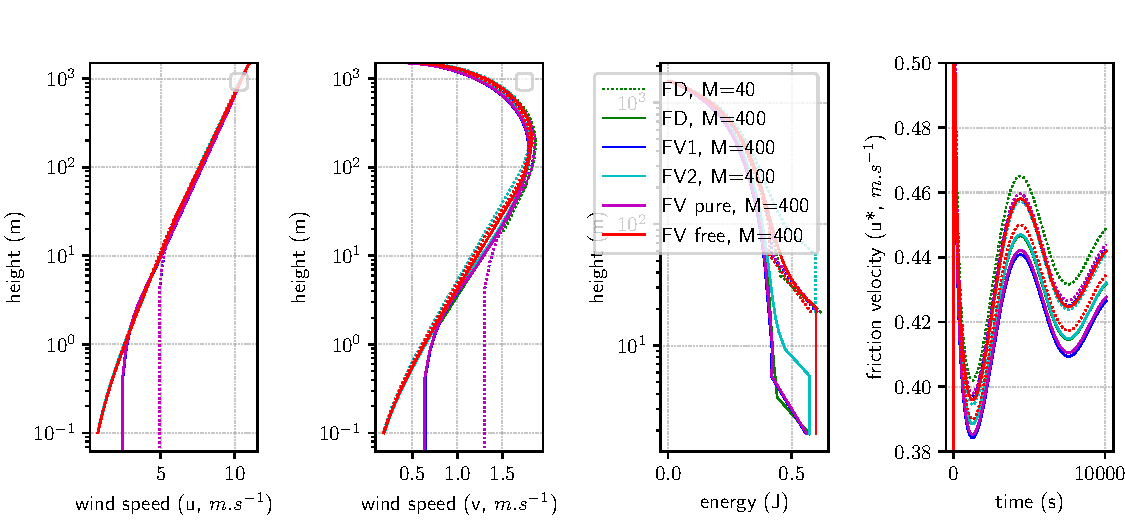
\includegraphics[scale=0.55]{images/consistency_comparison.pdf}
% 	\includegraphics[scale=0.55]{images/consistency_comparison_linearscale.pdf}
% 	\caption{Neutral case's numerical experiment. Top: log-scaled, bottom: linear-scaled}
% 	\label{fig:ND_NeutralCase_NumericalExp}
% \end{figure}
% \subsection{Variation of $\delta_{\rm sl}$}
% In this subsection we assume that $\delta_{\rm sl}$ can differ
% from one time to another. Let us note
% $\delta_{\rm sl}^n, \delta_{\rm sl}^{n+1}$ the two different sizes
% of the surface layer.
% There are 3 cases to take into account:
% \begin{enumerate}
% \item there is a $k$ such that
% 	$z_k< \delta_{\rm sl}^n, \delta_{\rm sl}^{n+1} < z_{k+1}$
% \item there is a $k$ such that
% 	$ \delta_{\rm sl}^n < z_k < \delta_{\rm sl}^{n+1}$
% \item there is a $k$ such that
% 	$ \delta_{\rm sl}^n > z_k > \delta_{\rm sl}^{n+1}$
% \end{enumerate}
% Note that multiple grid levels can be between $\delta_{\rm sl}^{n}$
% and $\delta_{\rm sl}^{n+1}$ in the second and third cases.
% \par
% Let $k^n$ be such that $z_{k^n} < \delta_{\rm sl}^{n}< z_{k^n + 1}$
% and $k^{n+1}$ such that
% $z_{k^{n+1}} < \delta_{\rm sl}^{n+1}< z_{k^{n+1} + 1}$
% \begin{enumerate}
% 	\item $k^n = k^{n+1}$:
% Since $\delta_{\rm sl}$ changes, then $\widetilde{h}$ also change.
% It must be taken into account when
% discretising in time the equations
% \eqref{eq:ND_NeutralCase_prognosticEqFVfree} and 
% \eqref{eq:ND_NeutralCase_semiDiscreteEkmanEqFVfree}.
% The boundary condition stays \eqref{eq:ND_NeutralCase_boundaryCondFVfree}.
% 	\item $k^n < k^{n+1}$:
% \eqref{eq:ND_NeutralCase_boundaryCondFVfree},
% \eqref{eq:ND_NeutralCase_prognosticEqFVfree} and 
% \eqref{eq:ND_NeutralCase_semiDiscreteEkmanEqFVfree} only need to
% be satisfied between $z_{k^{n+1}}$ and $z_{k^{n+1}+1}$.
% Hence, $\tau_{sl}(t^n)$ is set to 0.
% 	\item $k^n > k^{n+1}$:
% \eqref{eq:ND_NeutralCase_prognosticEqFVfree} and 
% \eqref{eq:ND_NeutralCase_semiDiscreteEkmanEqFVfree}
% need to be satisfied in both cells.
% {\color{red} It is not possible to do this in a natural way,
% because using \eqref{eq:ND_NeutralCase_prognosticEqFVfree}
% assumes the solution was a quadratic spline whereas it was actually
% a log profile.
% }
% \end{enumerate}
\paragraph{On the value of $K_{u,0}$}
\label{sec:ND_StratifiedCase_viscosity0_FVpure}
According to the wall law $K_{u,0}$ should be equal to $K_{mol}$.
However, the boundary condition $K_{u,0} \phi_0 = u_\star^2 e_\tau$
does not behave the same way with Finite Differences and Finite
Volumes.
\begin{itemize}
	\item \textbf{Finite Differences}:
Injecting the boundary condition in the first grid level gives
		\begin{equation}
			\partial_t u_{1/2} = \frac{1}{h_{1/2}}
			\left(K_{u,1}\frac{u_{3/2} - u_{1/2}}{h_1}
			 - u_\star^2 e_\tau \right).
		\end{equation}
The value of $K_0$ does not intervene in the equation.
\item \textbf{Finite Volumes} ("FV pure" and "FV1"):
In the continuity equation at $z=z_1$, it is implicitly used that
	\begin{equation}
		\partial_t u(z_1) =
		\frac{K_{u,1} \phi_1 - u_\star^2 e_\tau} {h_{1/2}}
		+ \frac{h \phi_1}{3}
		+ \frac{h u_\star^2 e_\tau}{6 K_{u,0}}
	\end{equation}
The (small) value of $K_{u,0}$ directly appears when we assume the
parabolic profile inside the first grid level.
As a result, $\partial_t u(z_1)$ scales with $\frac{1}{K_0}$ and
as it is seen in Figure \ref{fig:ND_NeutralCase_comparisonPlot}
exhibits unreasonable values.
To obtain physically plausible profiles,
by copying the expression $\phi_{\delta} = \frac{K_{mol}}{K_{u,\delta}}\phi_0$ of the "FV free" scheme, the surface
viscosity will be multiplied by $\frac{K_{u,\delta}}{K_{mol}}$.
However, it does not correspond to the original discretisation choice.
The consequence is that $\phi_0$ really corresponds
to neither $(\partial_z u)(z_0)$ nor $(\partial_z u)(z_{\delta_{sl}})$.
{\color{red} J'aimerais avoir une idée de si ce genre de trucs
		arrive dans des modèles + sophistiqués}
\end{itemize}

\paragraph{In the general case where $\delta_{\rm sl} \geq z_k$.}
Let $k$ be such that $z_k \leq \delta_{\rm sl} < z_{k+1}$.
The surface layer scheme "FV free" is identical to the case $k=0$, except that
\begin{itemize}
	\item the sub-cell of average $\widetilde{u}$ and of size
		$\widetilde{h}$ is $[\delta_{\rm sl}, z_{k+1}]$:
		$k$ is added to the indices in 
		\eqref{eq:ND_NeutralCase_boundaryCondFVfree} and
		\eqref{eq:ND_NeutralCase_semiDiscreteEkmanEqFVfree};
	\item $\tau_{sl} = \frac{1}{{h_{1/2}}}\int_{z_k}^{\delta_{sl}} \frac{\ln(1+\frac{z}{z_{u}})}{\ln(1+\frac{\delta_{sl}}{z_{u}})} dz$ and $\alpha_{\rm sl} = \frac{\widetilde{h}}{h_{k+1/2}} + \tau_{\rm sl}$;
	\item for $m < k$, the cell $[z_m, z_{m+1}]$ is filled with
		$K_{u,m} \phi_m = K_{u,k}\phi_k =
	{u_\star}^2e_\tau$
		and the average $\overline{u}_{m+1/2}$
		is computed with the integrated wall law
		between $z_m$ and $z_{m+1}$.
		The subgrid reconstruction in those cells are directly
		the wall law.
\end{itemize}
It is straightforward to check that for $\delta_{sl} = z_1$
the "FV2" scheme is rigorously recovered.
The derivation for any $\delta_{\rm sl} \geq 0$ is detailed for
the stratified case in section \ref{sec:ND_StratifiedCase_FVfree}
\begin{figure}
	\subimport{images/}{nouvelle_dis_neutre_anydelta.pdf_tex}
	\caption{ Surface layer scheme "FV free" with
	$\delta_{sl} \geq z_k$.}
	\label{fig:ND_NeutralCase_nouvelle_dis_neutre_anydelta}
\end{figure}
Figure \ref{fig:ND_NeutralCase_nouvelle_dis_neutre_anydelta}
shows how is handled the surface layer in this case: the part in gray
is neutralized for the prognostic equation and is filled afterward
with the help of the log law.
